\documentclass[hyperref={pdfpagelabels=false}]{beamer}
\usepackage{lmodern}
\usepackage{amsmath}
\usepackage{graphicx}
\usepackage{mathptmx} % seems something to do with the font

\usetheme{Frankfurt}
\setbeamercolor{section in head/foot}{fg=white, bg=blue!30!black!90}

\newcommand\mynew{andyandyandy}

%% configuration for the slids style
\makeatletter
\setbeamertemplate{footline}
{
  \leavevmode%
  \hbox{%
    \begin{beamercolorbox}[wd=.333333\paperwidth,ht=2.25ex,dp=2ex,center]{author in head/foot}%
      \usebeamerfont{author in
        head/foot}%
      \insertshortauthor\hspace{1em}\beamer@ifempty{\insertshortinstitute}{}{(\insertshortinstitute)}
    \end{beamercolorbox}%
    \begin{beamercolorbox}[wd=.333333\paperwidth,ht=2.25ex,dp=2ex,center]{title in head/foot}%
      \usebeamerfont{title in head/foot}\insertshorttitle
    \end{beamercolorbox}%
    \begin{beamercolorbox}[wd=.333333\paperwidth,ht=2.25ex,dp=2ex,right]{date in head/foot}%
      \usebeamerfont{date in head/foot}\insertshortdate{}\hspace*{2em}
      \insertframenumber{} / \inserttotalframenumber\hspace*{2ex}
    \end{beamercolorbox}}%
  \vskip0pt%
}
\makeatother

\author[\parbox{.2\paperwidth}{}]{Hu SiXing, Hakki Can Karaimer, Pan An, Philipp Keck}
\institute{National University of Singapore}
\title{Convex Optimization}

%% end of configuration




% \title{Convex Optimization}
% \author{Hu SiXing, Hakki Can Karaimer, Pan An, Philipp Keck}
% \date{\today}
\begin{document}

\begin{frame}
  \titlepage
\end{frame}


% \begin{frame}
%   % \frametitle{Table of contents}
%   % \tableofcontents
% %%% Local Variables:
%%% mode: latex
%%% TeX-master: t
%%% End:

%%  commands definition and some other definitions about stuffs
\newcommand\here{lalala}
%\newcommand\x{x_i}
%\newcommand\y{y_i
\newcommand\dis{\displaystyle }


\subsection{}
\begin{frame}
  \frametitle{Linear Regression Example}
  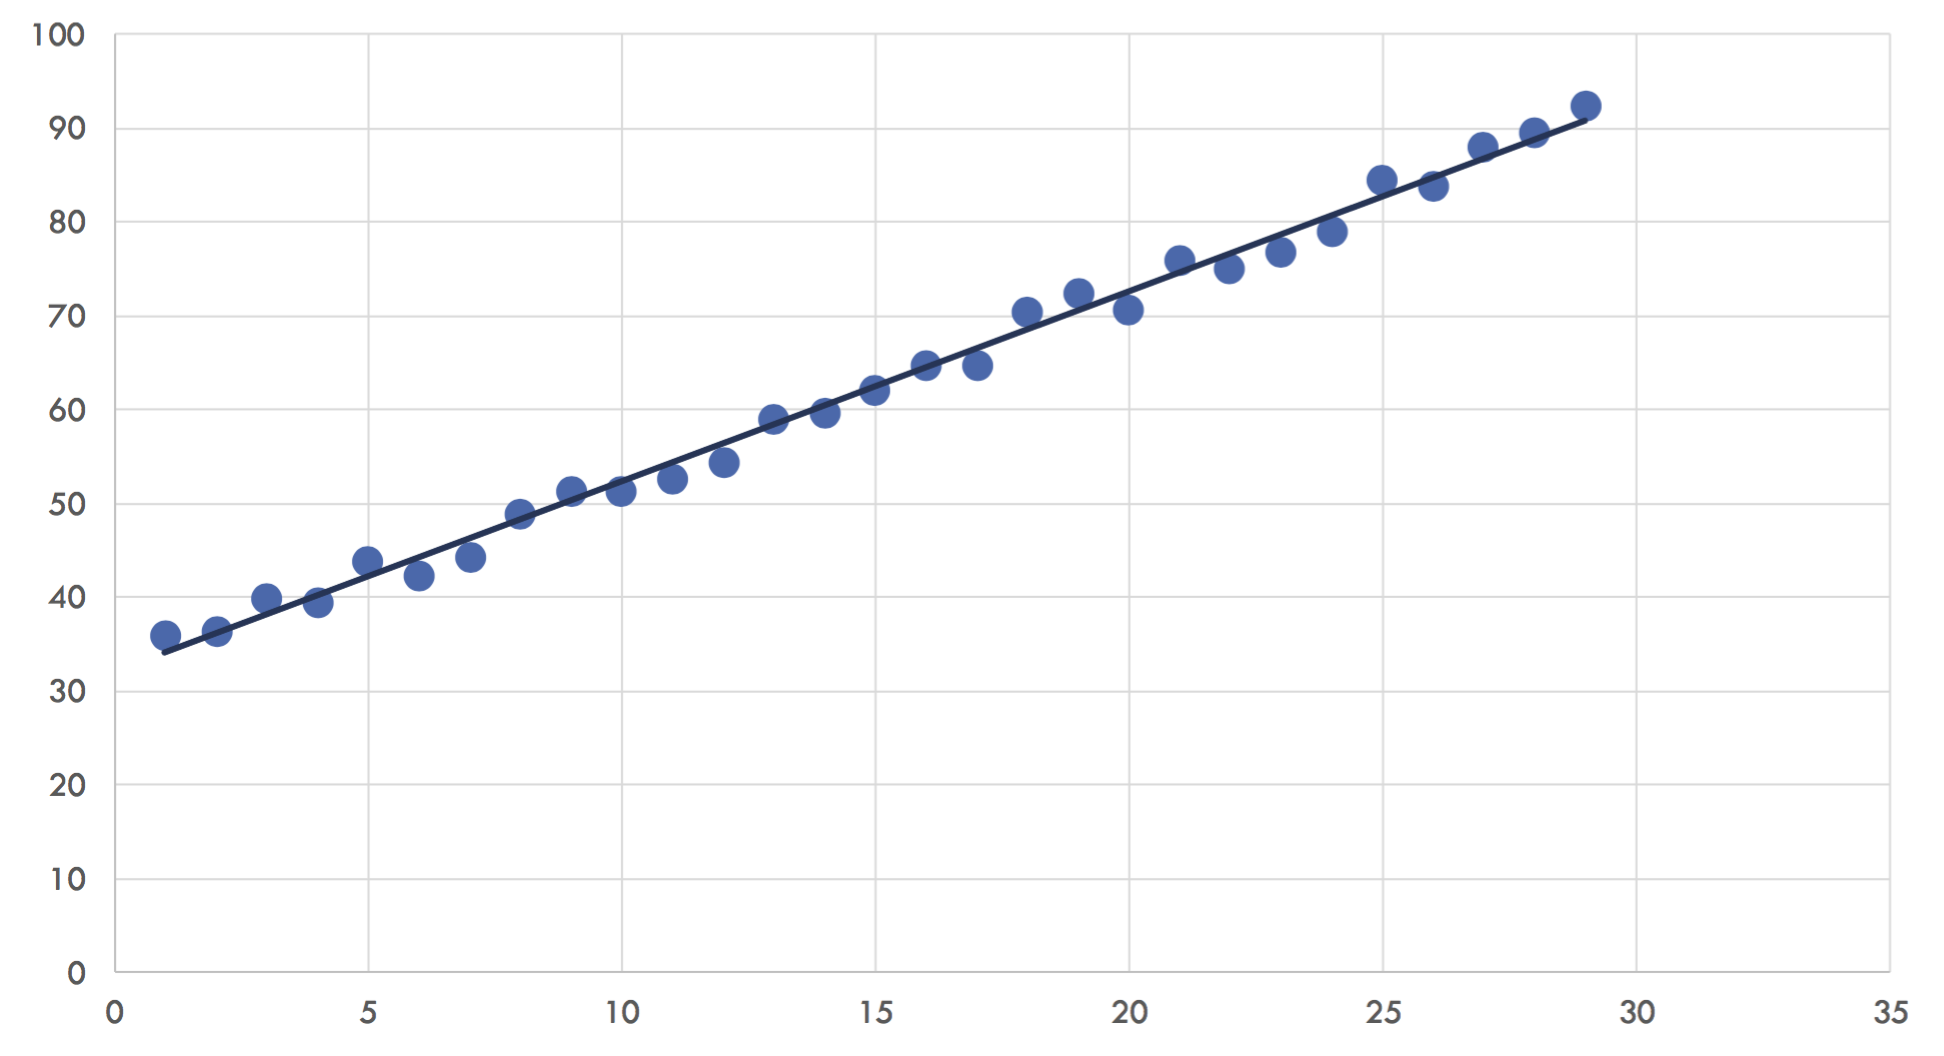
\includegraphics[scale=0.32]{pics/linear.png}

\end{frame}


\subsection{}
\begin{frame}
\frametitle{Ordinary Least Squares}

% 2 columns examples
\begin{columns}
  \begin{column}{0.6\textwidth}
    \begin{itemize}
    \item[] Input: points $(x_i, y_i)$
      \item[] Regression line: $y = mx + b$
\item[] Objective: $\displaystyle \min_{m, b} \sum_{i}(y_i - mx_i -b)^2$
    \end{itemize}
  \end{column}

  \begin{column}{0.5\textwidth}
    \begin{itemize}
    \item[] $(\vec{x_i}, y_i)$
    \item[] $y = \vec{w} \cdot \vec{x} + b$
    \item[] $\dis \min_{\vec{w}}\sum_{i}(y_i - \vec{w} \cdot \vec{x_i} -b)^2$
    \end{itemize}

  \end{column}
\end{columns}

\begin{itemize}
\item Easily Solved: $\vec{w}^*(X^TX)-X^T\vec{y}$
\item But what if $\dim\vec{x} $ is large?
\item What about other similar regressions?
\end{itemize}

\end{frame}

\subsection{}
\begin{frame}
\frametitle{Convex Optimization Problems}


\begin{itemize}
\item OrdinaryLinearRegression: $\dis \min_{\vec{w}}\sum_i(y_i -
  \vec{w} \cdot \vec{x_i})^2$
\item General: $\dis \min_xf(x)$ where $f(x)$ is convex
\item Set $C$ is convex $\Longleftrightarrow \forall x, y\in C, 0\le t
  \le 1: tx +(1 - t)y \in C$
\item Function $f : \mathbb{R}^n \rightarrow \mathbb{R}$ is convex if
  $\dom f$ is convex and $\exists x, y \in \dom f, 0\le t \le 1:$

\end{itemize}

\vspace{-4mm}

{\small
$$f(tx + (1 - t)y) \le tf(x) + (1 - t)f(y)$$
}

\vspace{-4mm}

\begin{columns}
  \begin{column}{0.5\textwidth}

\begin{itemize}
\item Unconstrained.
\end{itemize}

  \end{column}

  \begin{column}{0.5\textwidth}
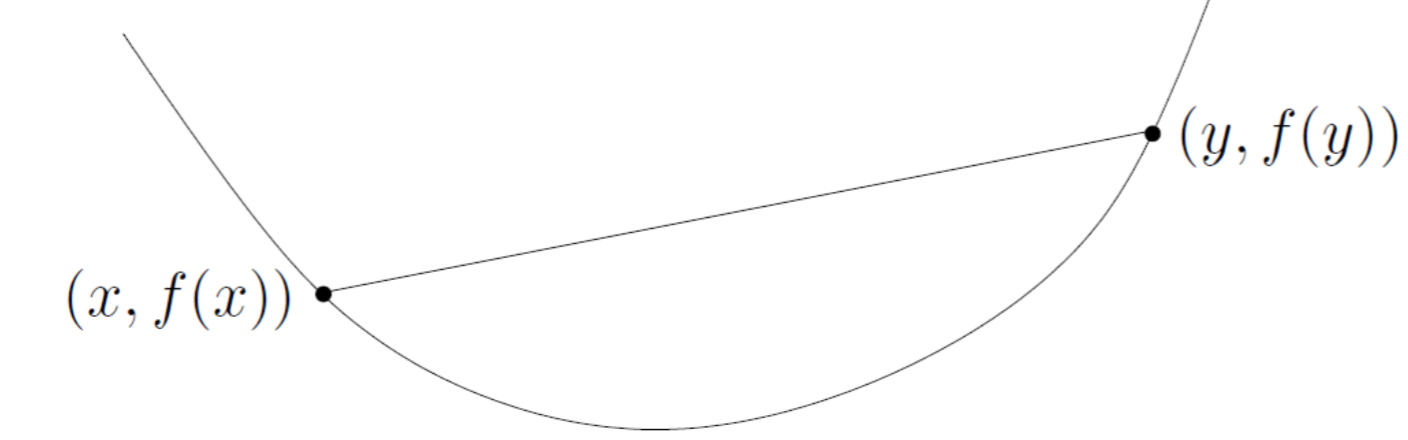
\includegraphics[scale=0.2]{pics/uncons.png}
  \end{column}
\end{columns}

\end{frame}

\subsection{}

\begin{frame}
  \frametitle{Outliers}
  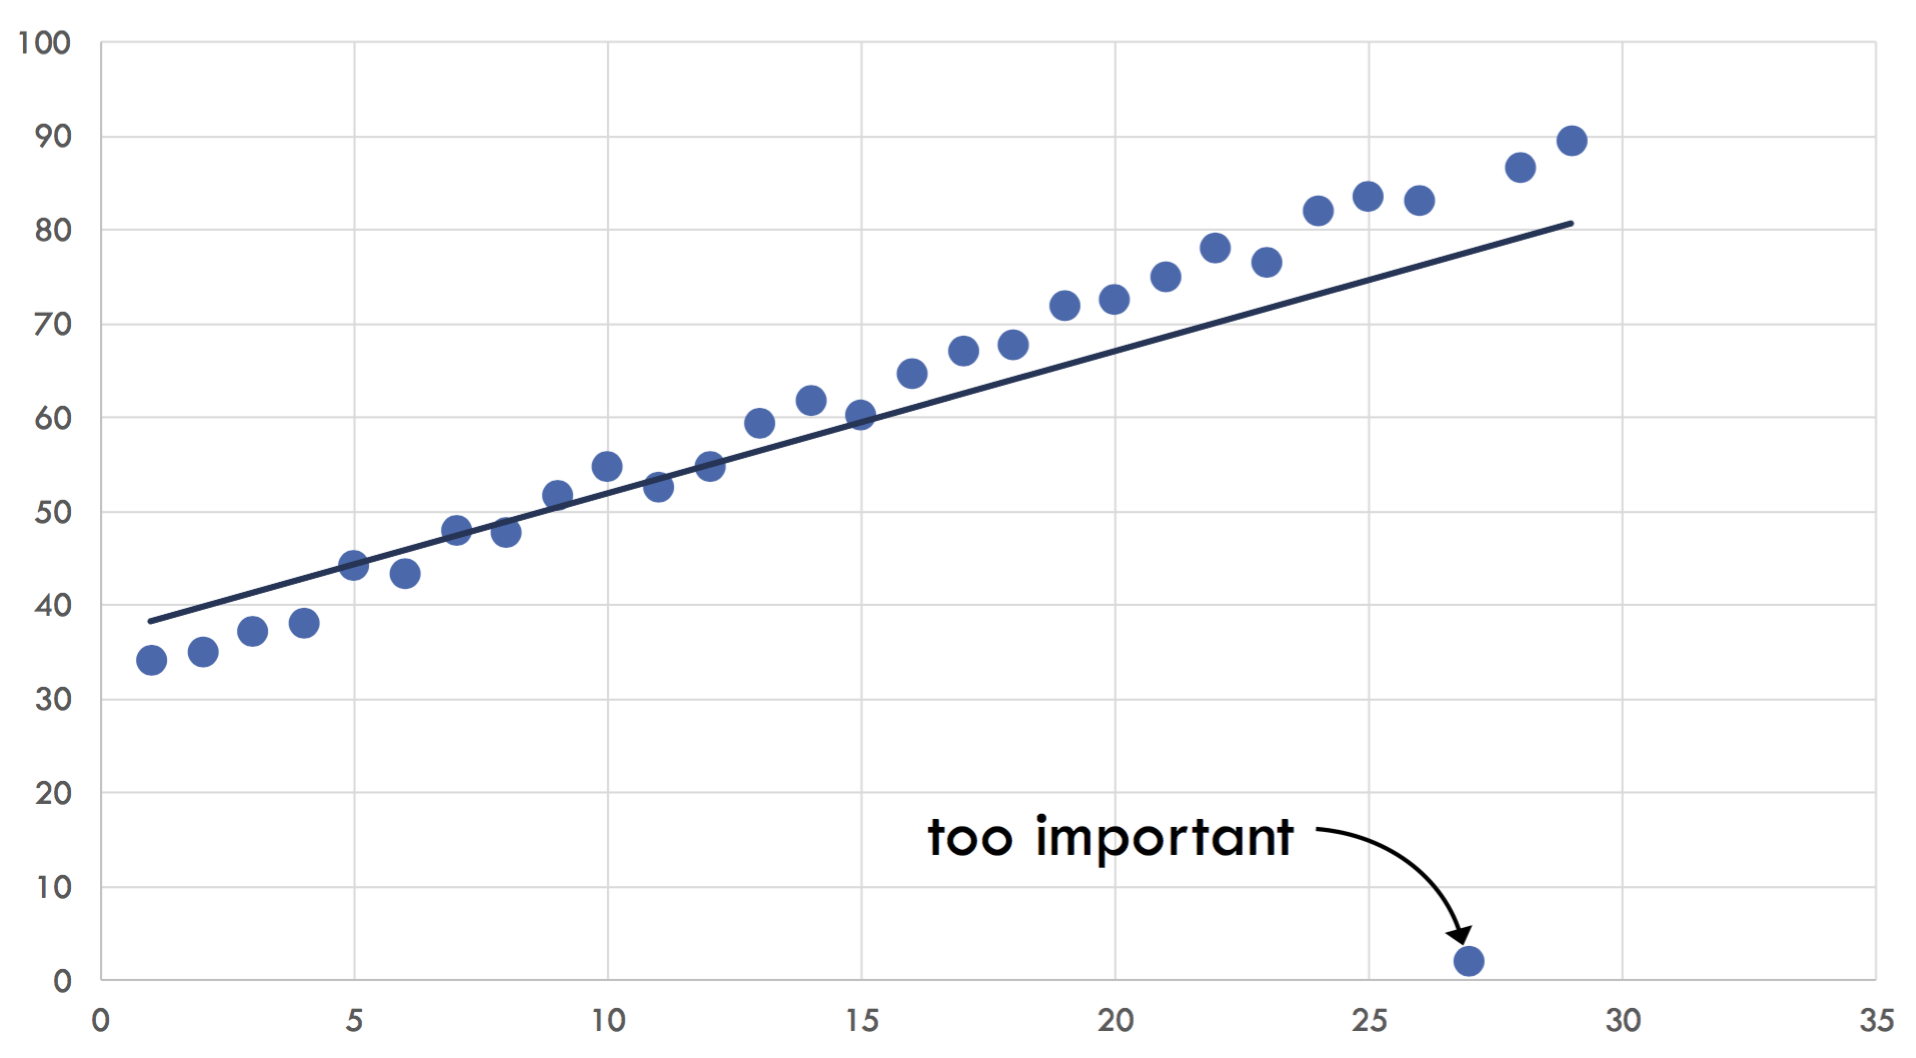
\includegraphics[scale=0.32]{pics/lpo.png}

\end{frame}

\subsection{}
\begin{frame}


  \frametitle{Outlier Penalty}

  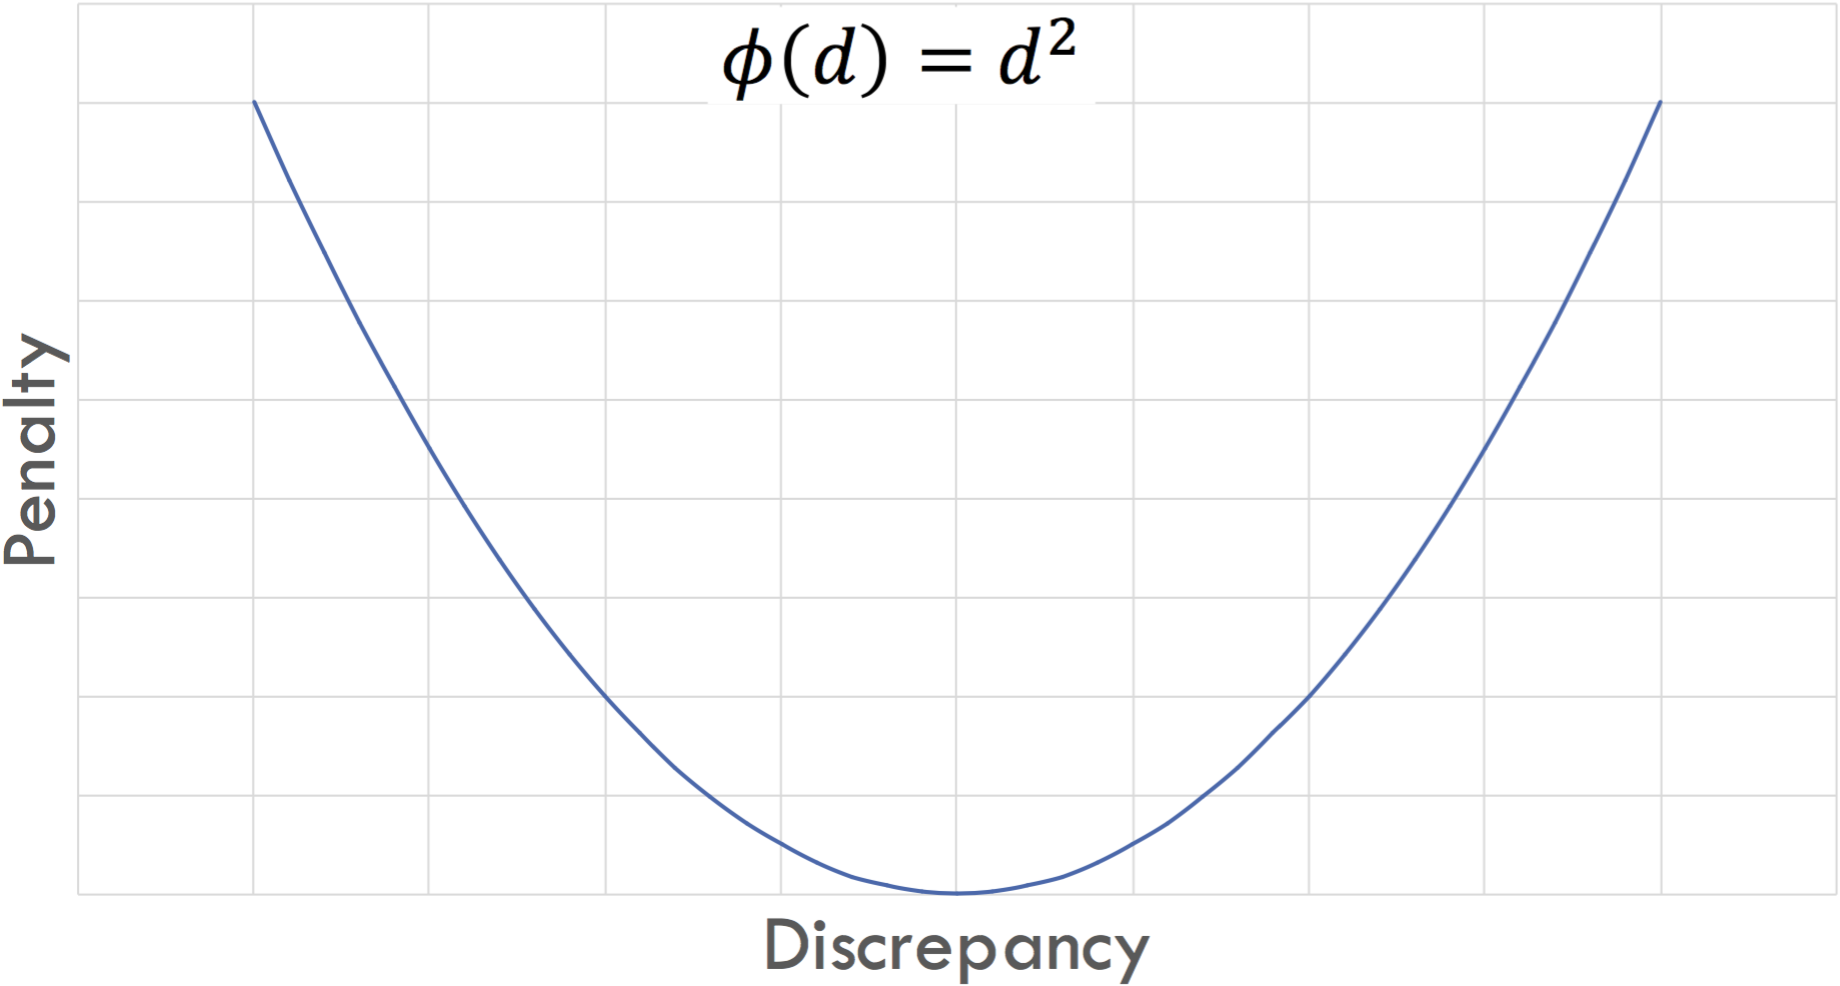
\includegraphics[scale=0.32]{pics/pen1.png}


\end{frame}

\begin{frame}
  \frametitle{Capped Penalty}
  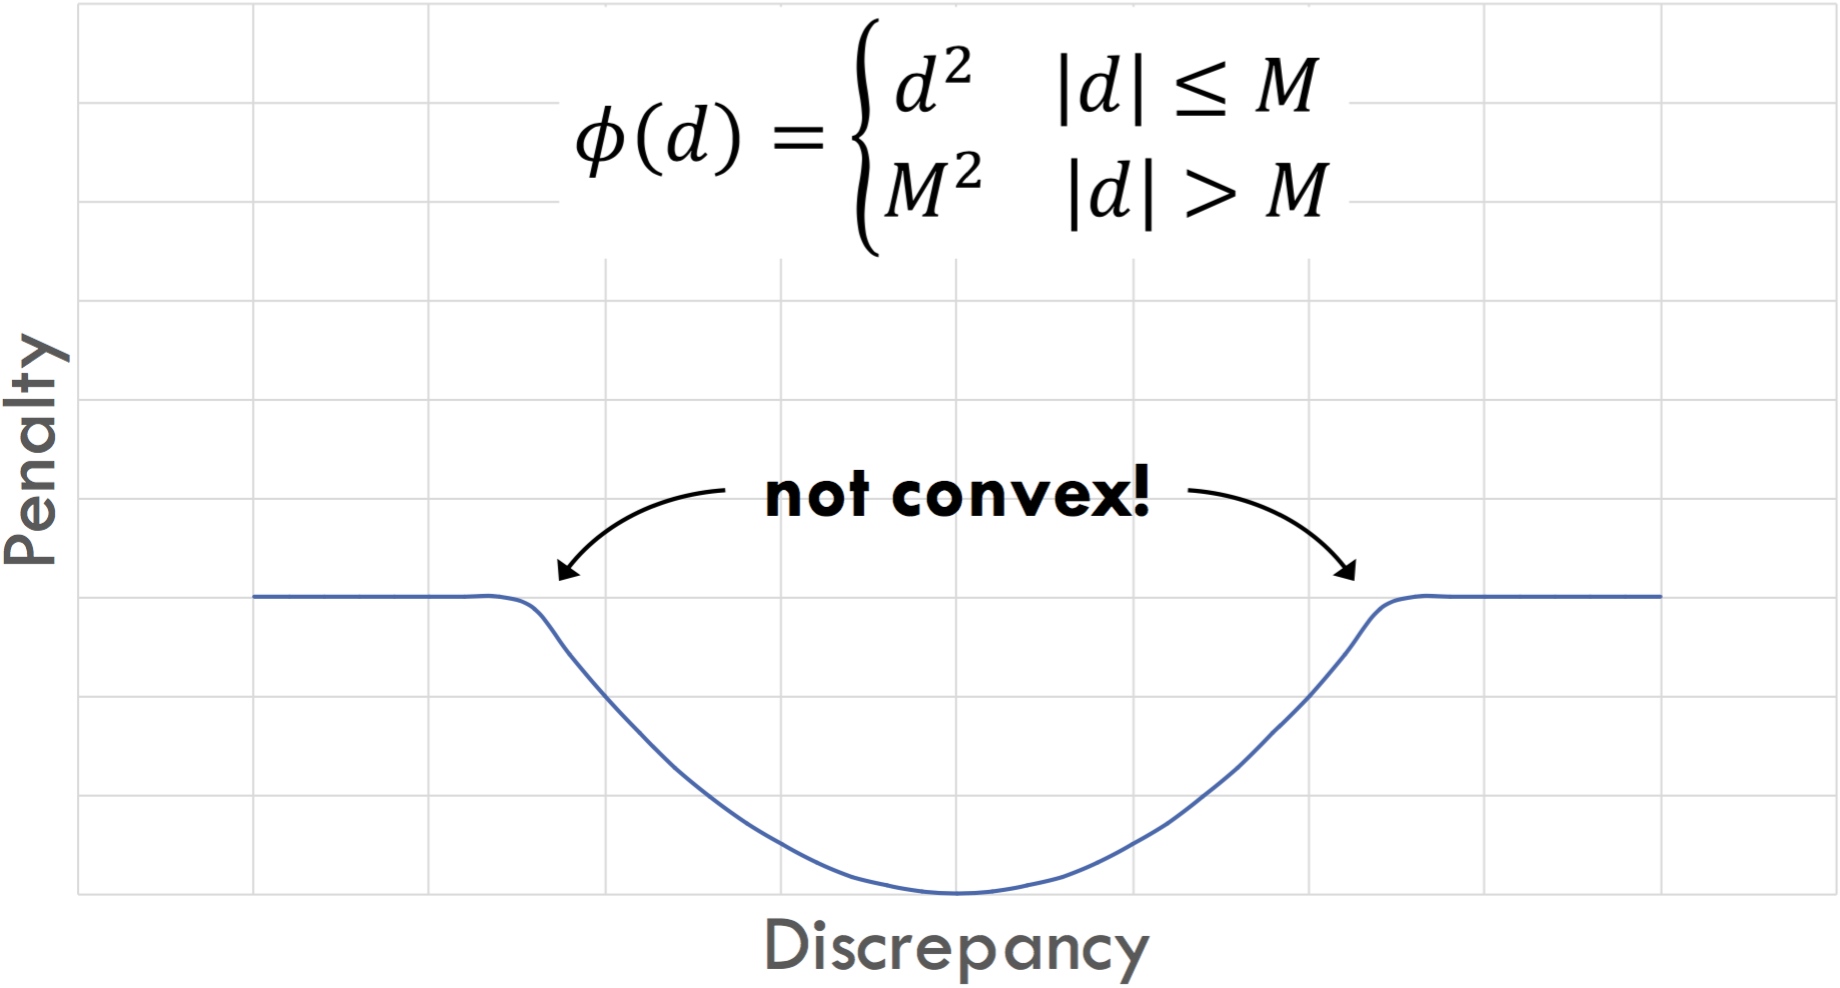
\includegraphics[scale=0.32]{pics/pen2.png}
\end{frame}

\begin{frame}
\frametitle{Huber Penalty Function}
  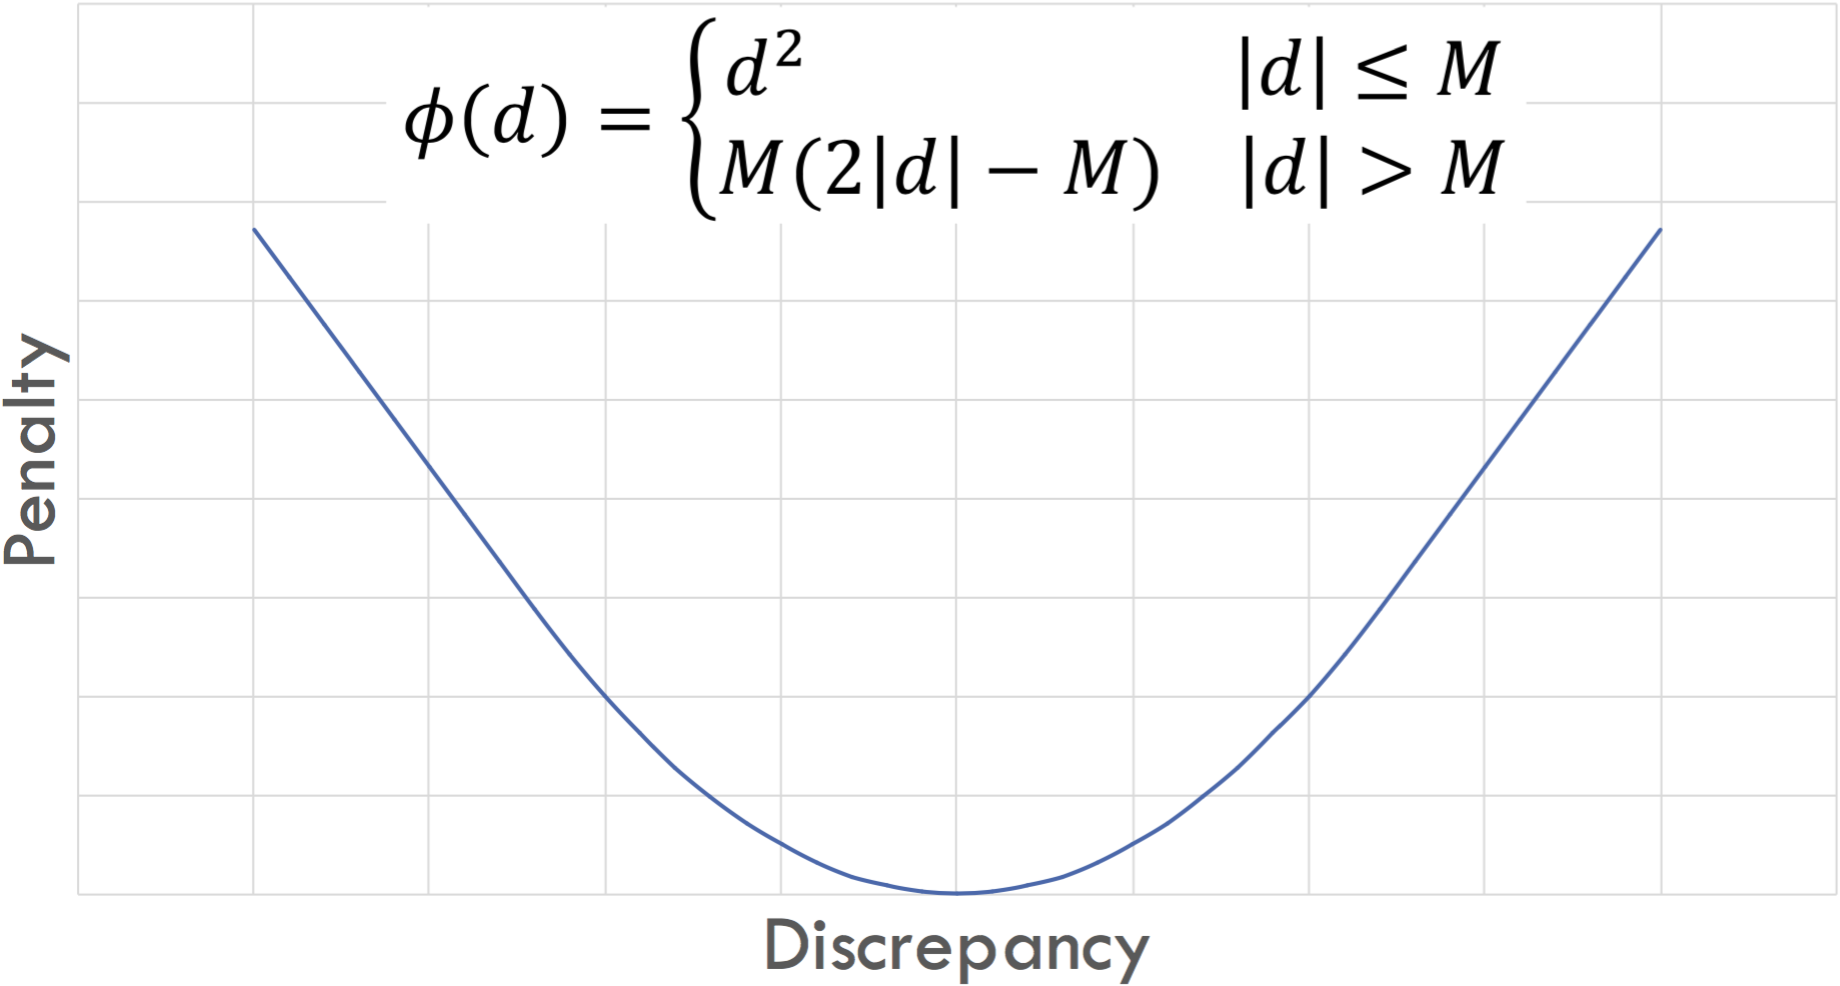
\includegraphics[scale=0.32]{pics/pen3.png}
\end{frame}

% \mynew
% \end{frame}


\section{Linear Regression}
%%% Local Variables:
%%% mode: latex
%%% TeX-master: t
%%% End:

%%  commands definition and some other definitions about stuffs
\newcommand\here{lalala}
%\newcommand\x{x_i}
%\newcommand\y{y_i
\newcommand\dis{\displaystyle }


\subsection{}
\begin{frame}
  \frametitle{Linear Regression Example}
  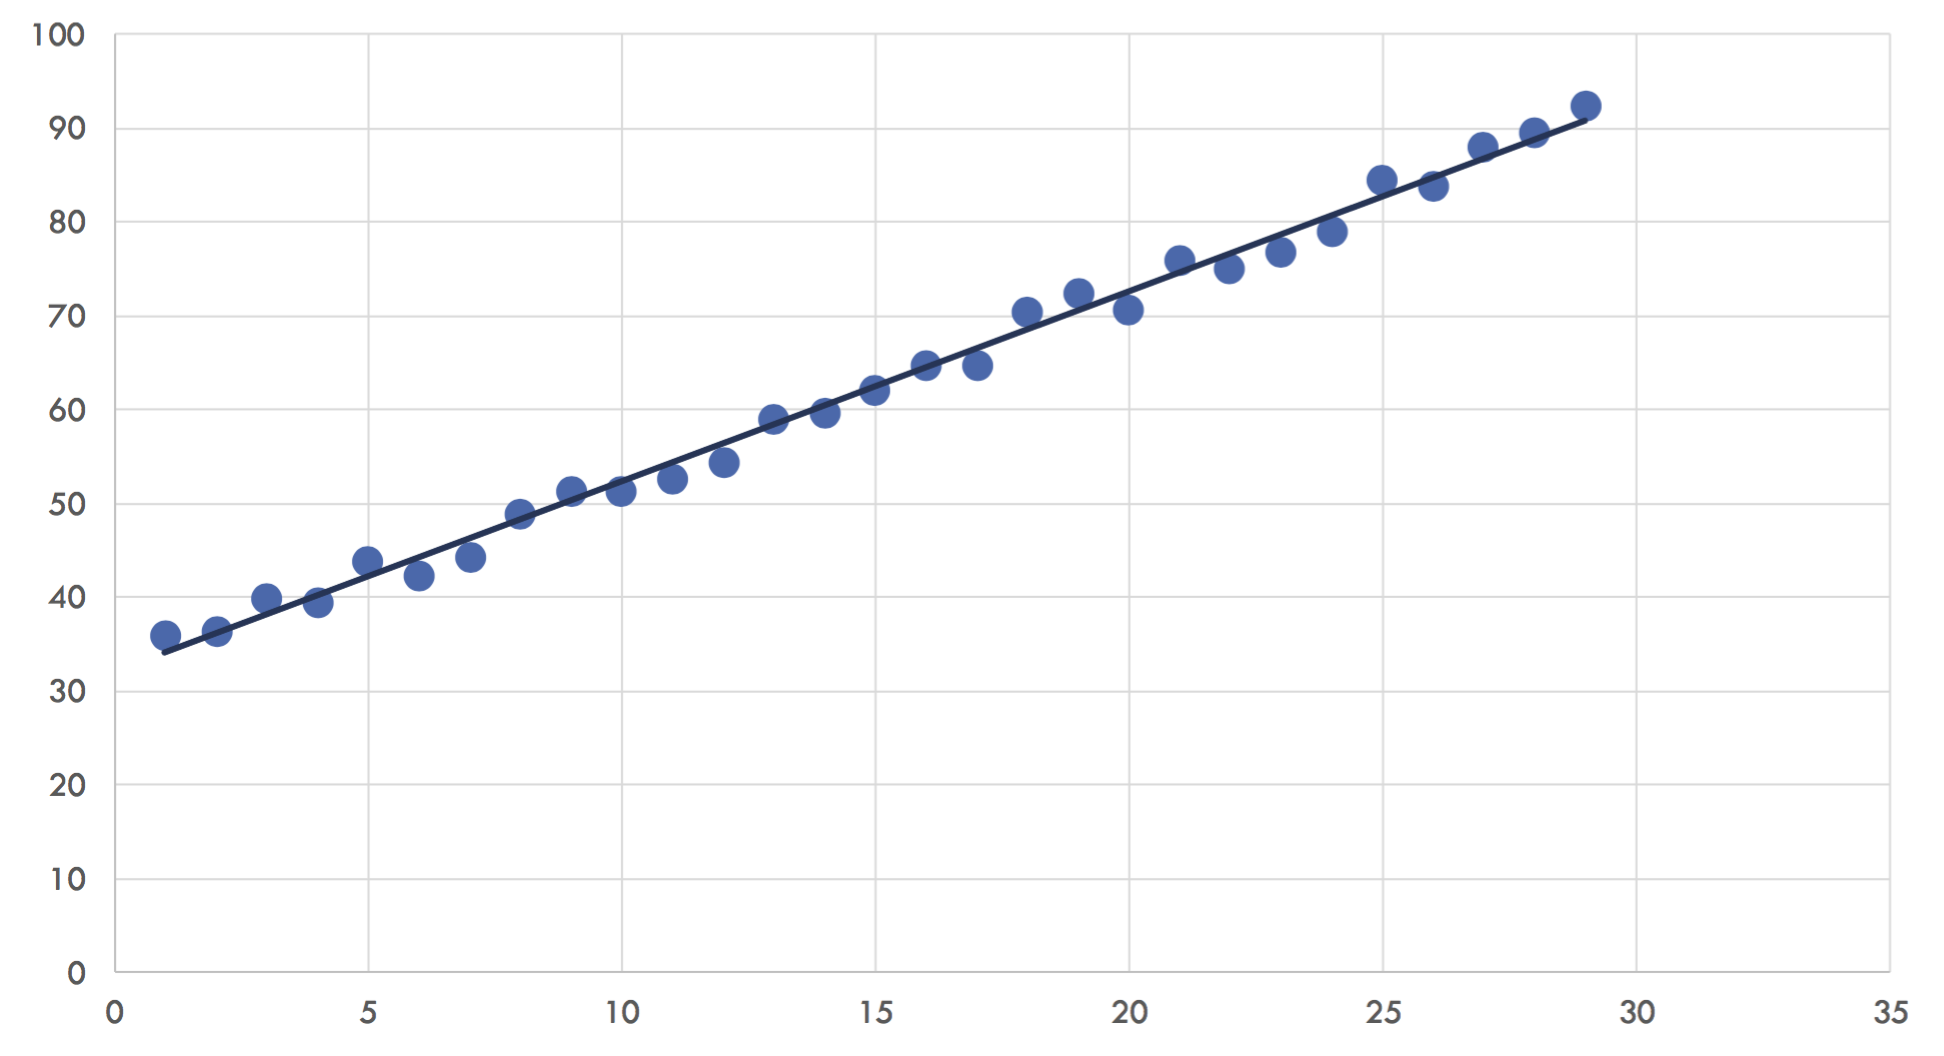
\includegraphics[scale=0.32]{pics/linear.png}

\end{frame}


\subsection{}
\begin{frame}
\frametitle{Ordinary Least Squares}

% 2 columns examples
\begin{columns}
  \begin{column}{0.6\textwidth}
    \begin{itemize}
    \item[] Input: points $(x_i, y_i)$
      \item[] Regression line: $y = mx + b$
\item[] Objective: $\displaystyle \min_{m, b} \sum_{i}(y_i - mx_i -b)^2$
    \end{itemize}
  \end{column}

  \begin{column}{0.5\textwidth}
    \begin{itemize}
    \item[] $(\vec{x_i}, y_i)$
    \item[] $y = \vec{w} \cdot \vec{x} + b$
    \item[] $\dis \min_{\vec{w}}\sum_{i}(y_i - \vec{w} \cdot \vec{x_i} -b)^2$
    \end{itemize}

  \end{column}
\end{columns}

\begin{itemize}
\item Easily Solved: $\vec{w}^*(X^TX)-X^T\vec{y}$
\item But what if $\dim\vec{x} $ is large?
\item What about other similar regressions?
\end{itemize}

\end{frame}

\subsection{}
\begin{frame}
\frametitle{Convex Optimization Problems}


\begin{itemize}
\item OrdinaryLinearRegression: $\dis \min_{\vec{w}}\sum_i(y_i -
  \vec{w} \cdot \vec{x_i})^2$
\item General: $\dis \min_xf(x)$ where $f(x)$ is convex
\item Set $C$ is convex $\Longleftrightarrow \forall x, y\in C, 0\le t
  \le 1: tx +(1 - t)y \in C$
\item Function $f : \mathbb{R}^n \rightarrow \mathbb{R}$ is convex if
  $\dom f$ is convex and $\exists x, y \in \dom f, 0\le t \le 1:$

\end{itemize}

\vspace{-4mm}

{\small
$$f(tx + (1 - t)y) \le tf(x) + (1 - t)f(y)$$
}

\vspace{-4mm}

\begin{columns}
  \begin{column}{0.5\textwidth}

\begin{itemize}
\item Unconstrained.
\end{itemize}

  \end{column}

  \begin{column}{0.5\textwidth}
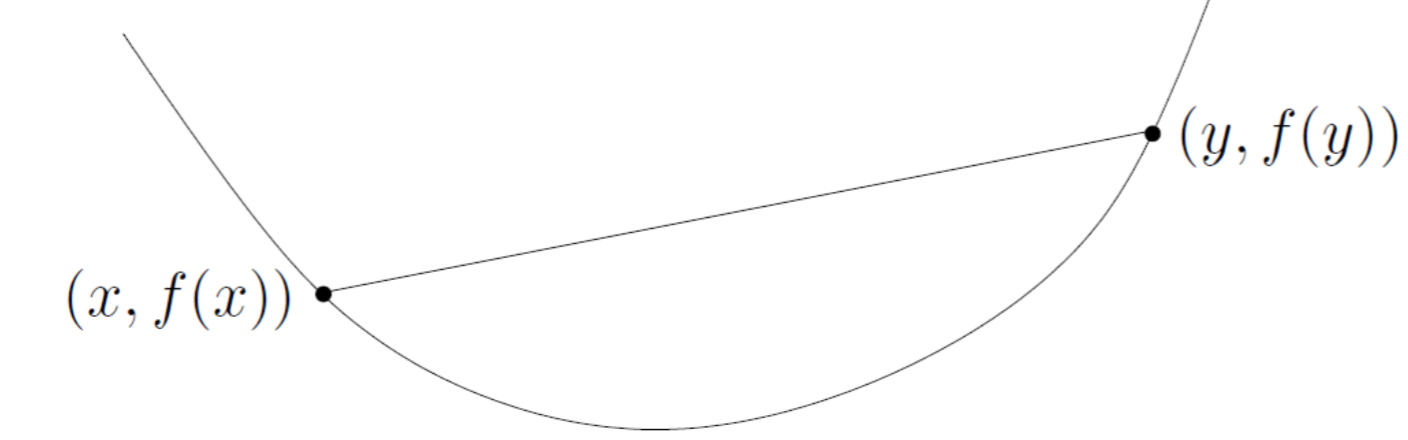
\includegraphics[scale=0.2]{pics/uncons.png}
  \end{column}
\end{columns}

\end{frame}

\subsection{}

\begin{frame}
  \frametitle{Outliers}
  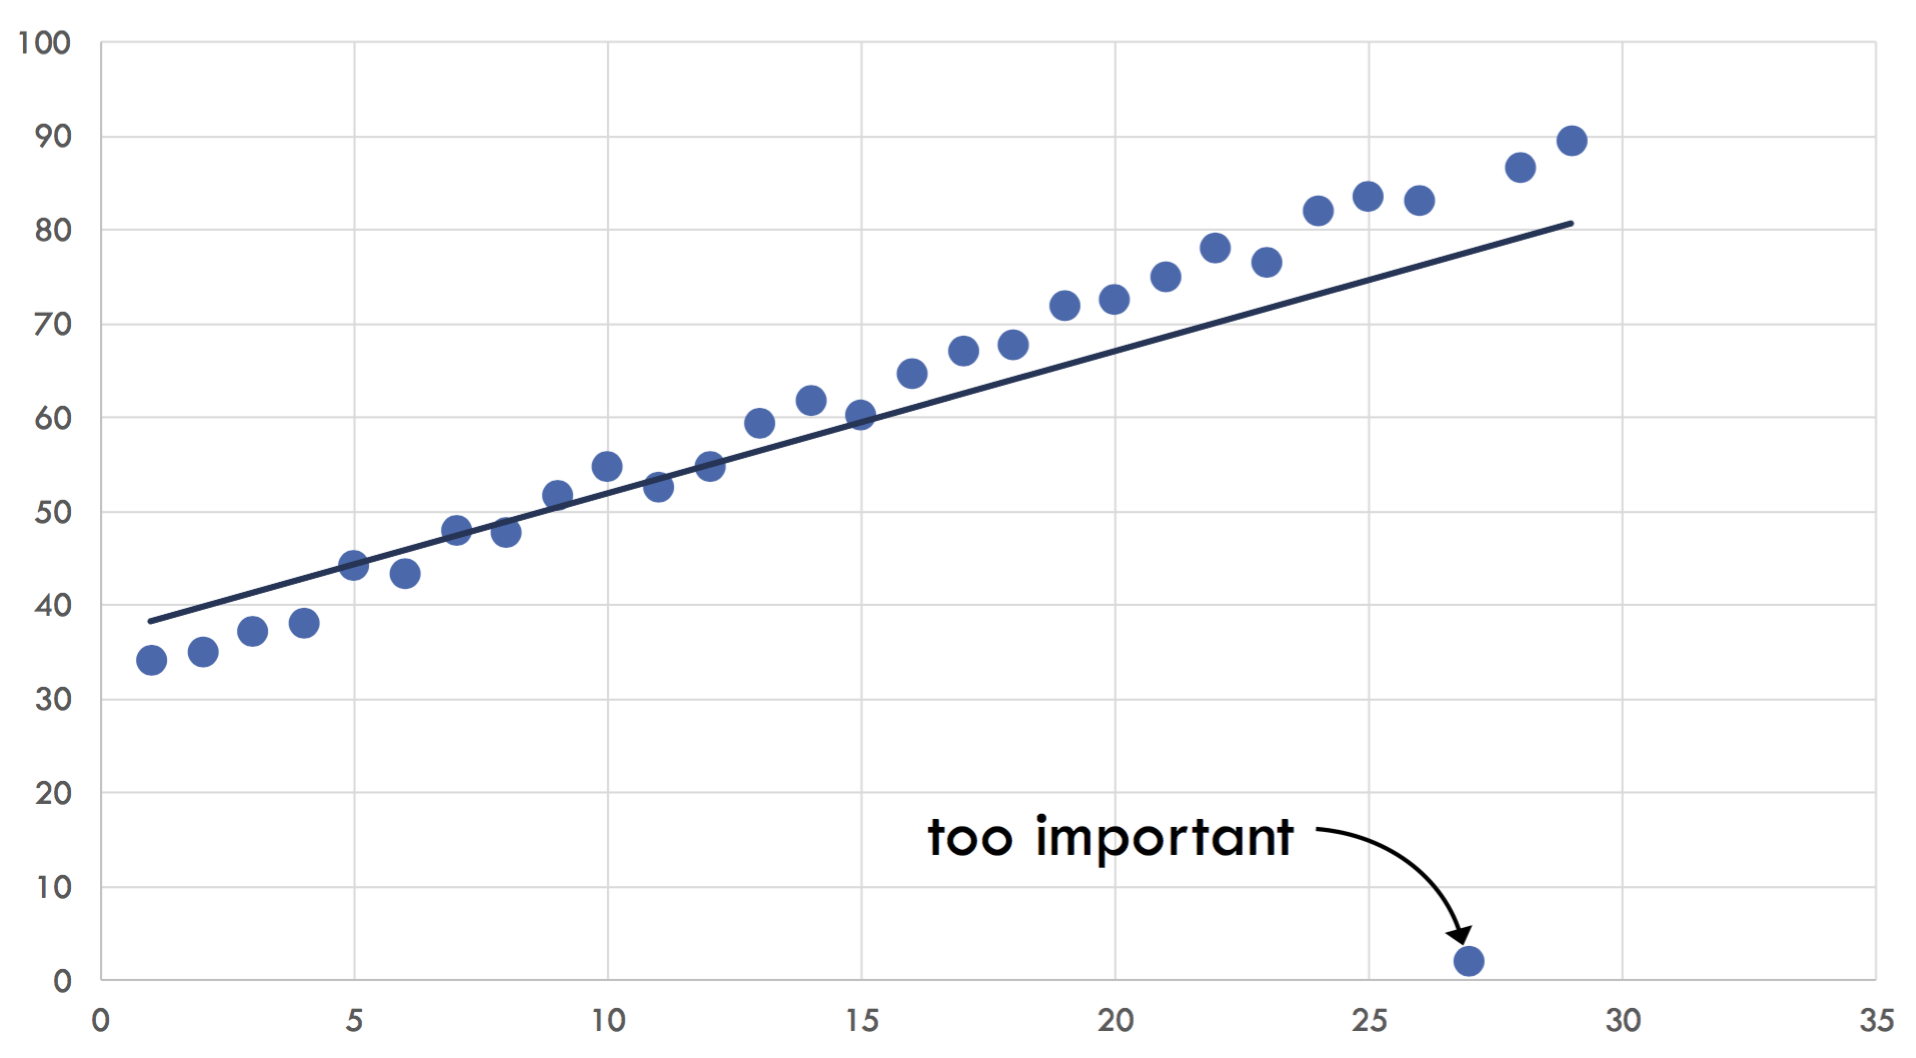
\includegraphics[scale=0.32]{pics/lpo.png}

\end{frame}

\subsection{}
\begin{frame}


  \frametitle{Outlier Penalty}

  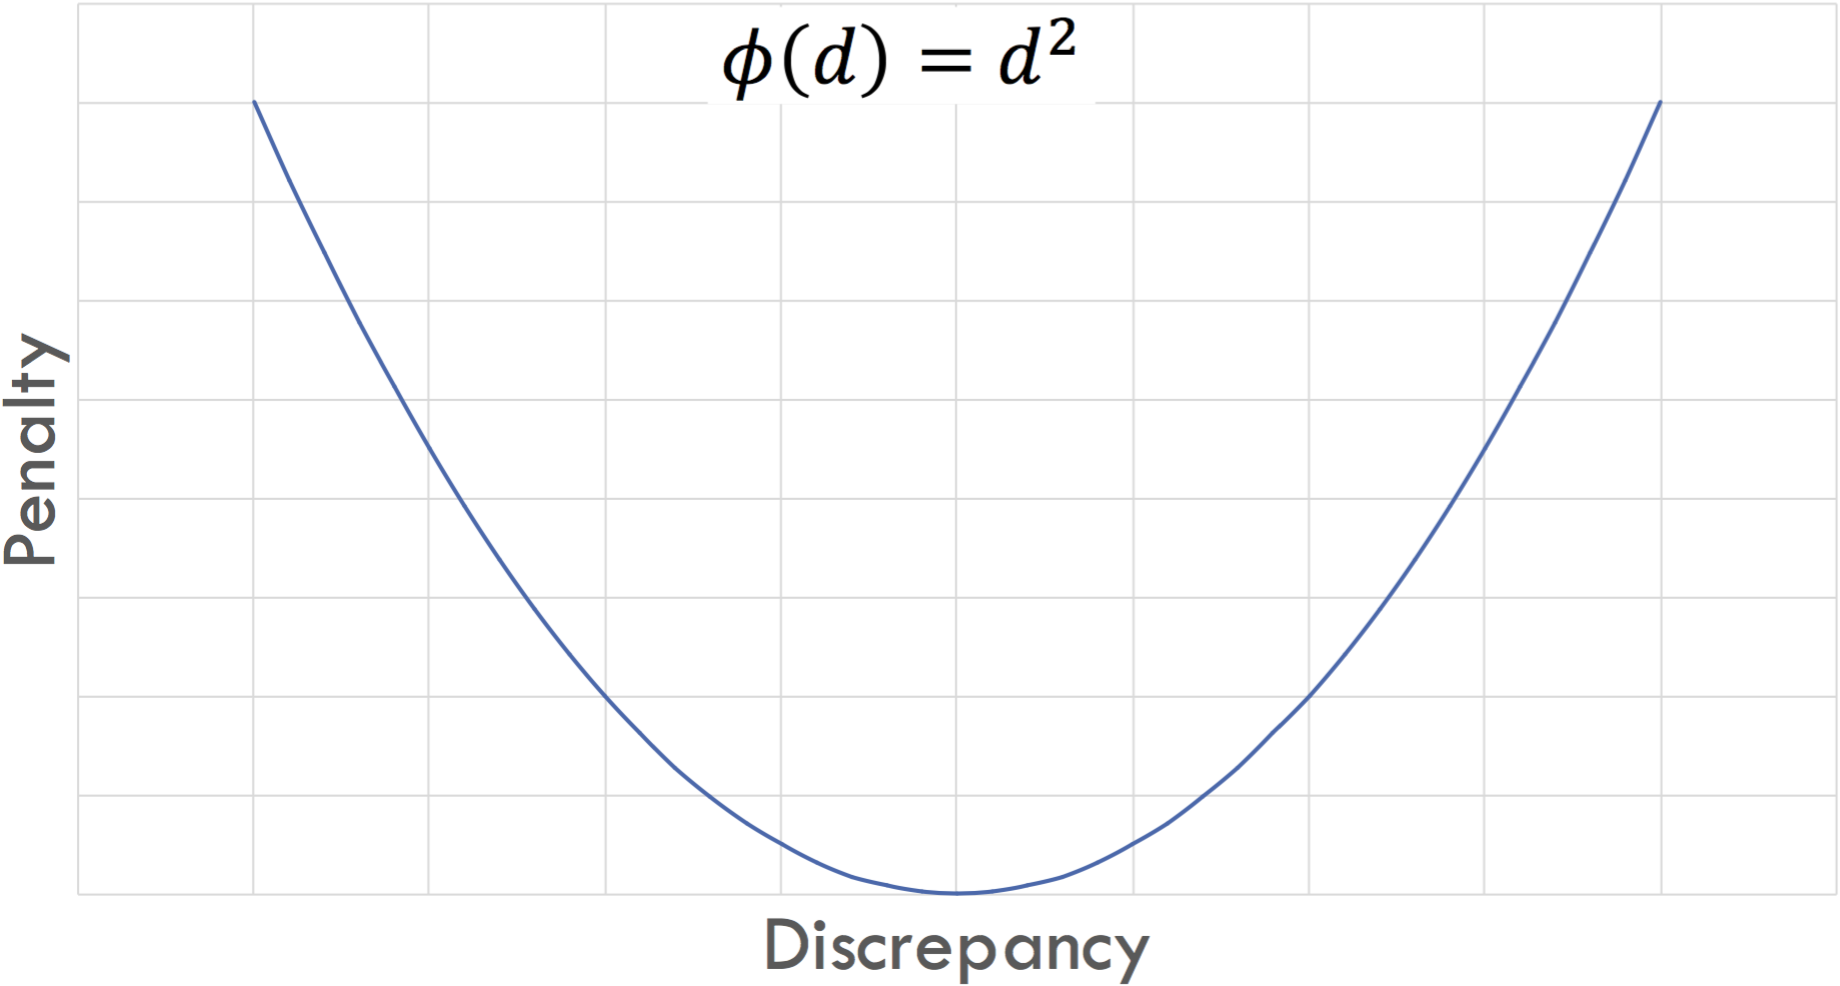
\includegraphics[scale=0.32]{pics/pen1.png}


\end{frame}

\begin{frame}
  \frametitle{Capped Penalty}
  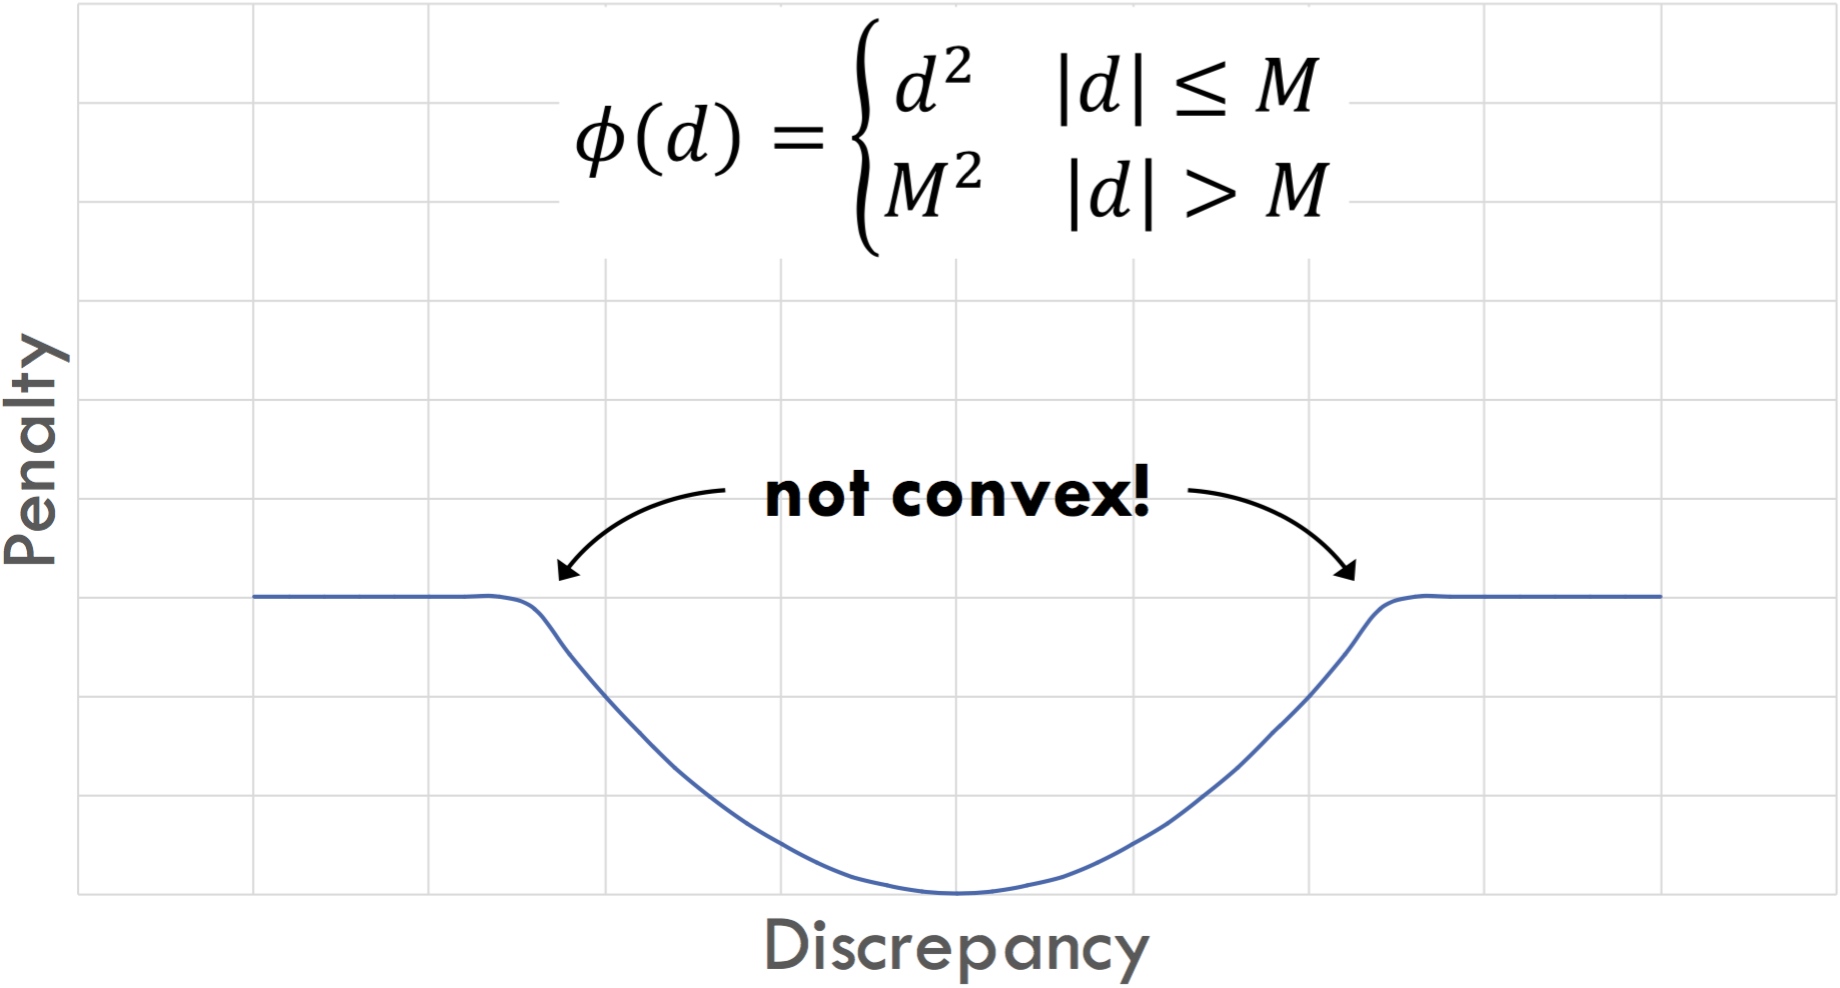
\includegraphics[scale=0.32]{pics/pen2.png}
\end{frame}

\begin{frame}
\frametitle{Huber Penalty Function}
  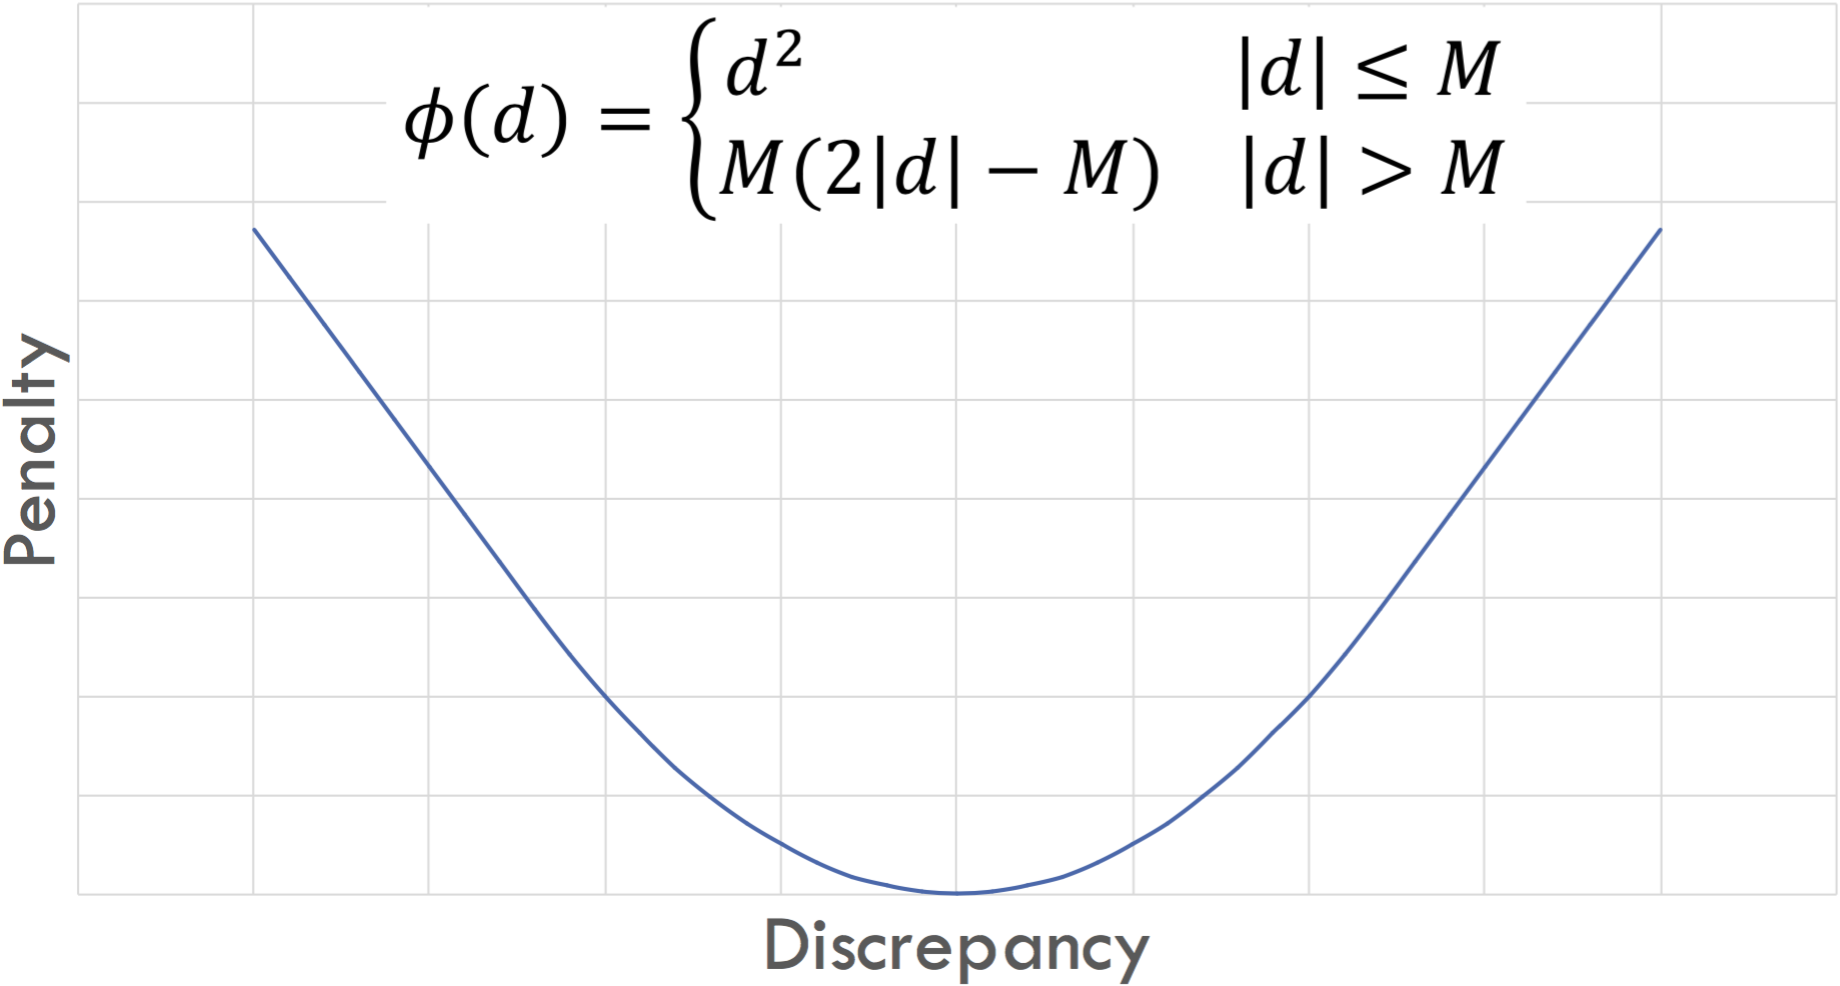
\includegraphics[scale=0.32]{pics/pen3.png}
\end{frame}



\section{Section no. 2}
\subsection{Lists I}
\begin{frame}
  \frametitle{unnumbered lists}
  \begin{itemize}
  \item Introduction to  \LaTeX{}
  \item Course 2
  \item Termpapers and presentations with \LaTeX{}
  \item Beamer class
  \end{itemize}
\end{frame}

\begin{frame}\frametitle{lists with single pauses}
  \begin{itemize}
  \item Introduction to  \LaTeX{}  \pause
  \item Course 2 \pause
  \item Termpapers and presentations with \LaTeX{}  \pause
  \item Beamer class
  \end{itemize}
\end{frame}

\begin{frame}\frametitle{lists with pause}
  \begin{itemize}[<+->]
  \item Introduction to  \LaTeX{}
  \item Course 2
  \item Termpapers and presentations with \LaTeX{}
  \item Beamer class
  \end{itemize}
\end{frame}



\subsection{Lists II}
\begin{frame}\frametitle{numbered lists}
  \begin{enumerate}
  \item Introduction to  \LaTeX{}
  \item Course 2
  \item Termpapers and presentations with \LaTeX{}
  \item Beamer class
  \end{enumerate}
\end{frame}

\begin{frame}
  \frametitle{numbered lists with single pauses}
  \begin{enumerate}
  \item Introduction to  \LaTeX{}  \pause
  \item Course 2 \pause
  \item Termpapers and presentations with \LaTeX{}  \pause
  \item Beamer class
  \end{enumerate}
\end{frame}

\begin{frame}
  \frametitle{numbered lists with pause}
  \begin{enumerate}[<+->]
  \item Introduction to  \LaTeX{}
  \item Course 2
  \item Termpapers and presentations with \LaTeX{}
  \item Beamer class
  \end{enumerate}
\end{frame}




\section{Section no.3}
\subsection{Tables}
\begin{frame}
  \frametitle{Tables}
  \begin{tabular}{|c|c|c|}
    \hline
    \textbf{Date} & \textbf{Instructor} & \textbf{Title} \\
    \hline
    WS 04/05 & Sascha Frank & First steps with  \LaTeX  \\
    \hline
    SS 05 & Sascha Frank & \LaTeX \ Course serial \\
    \hline
  \end{tabular}
\end{frame}


\begin{frame}
  \frametitle{Tables with pause}
  \begin{tabular}{c c c}
    A & B & C \\
    \pause
    1 & 2 & 3 \\
    \pause
    A & B & C \\
  \end{tabular}
\end{frame}


\section{Section no. 4}
\subsection{blocs}
\begin{frame}
  \frametitle{blocs}

  \begin{block}{title of the bloc}
    bloc text
  \end{block}

  \begin{exampleblock}{title of the bloc}
    bloc text
  \end{exampleblock}


  \begin{alertblock}{title of the bloc}
    bloc text
  \end{alertblock}
\end{frame}

\end{document}


%%% Local Variables:
%%% mode: latex
%%% TeX-master: t
%%% End:
